\documentclass[12pt]{article}
\usepackage{fullpage}
\usepackage[shortlabels]{enumitem}
\usepackage{amsmath}
\usepackage{amsthm}
\usepackage{graphicx}
\usepackage{amssymb}
\usepackage{enumitem}

\title{250 Homework $\#$4 (Fall 2026)}
\author{Toby Hansen \footnote{Collaborated with Nobody.}}
\begin{document}
	\date{}
	\maketitle

	This assignment is due at 11:59 p.m.~on Monday, 9 November 2026, to be submitted
	on Gradescope. Late assignments (with penalty, unless excused) will be accepted
	until 11:59 p.m. on Tuesday, 10 November 2026, and not after. Please see the syllabus
	for more details on homework grading and late penalties.

	\medskip

	When submitting to Gradescope, please do not forget to assign pages to problems.

	%\medskip

	% All problems, with the exception of the first two and ,  originally come from the textbook. Some of them have been modified.  In case of doubt, the version printed here is the one you should follow.

	\bigskip

	The formatting and submission guidelines are the same for this assignment as
	for the previous ones. Please see the Canvas Homework page for the complete guideline
	details.

	\medskip

	Many of the problems originally come from the textbook and have their original
	reference numbers, e.g., 4.4.8, attached. Many of those have been modified
	from the book version. In those cases, you should solve the version given here
	and not the original one in the book.

	% \medskip

	\medskip

	{\bf Special Induction Rules:} Important. Any problem that requires you to prove
	something by induction should be split into three distinct labelled parts:

	\begin{itemize}
		\item[(i)] State the induction hypothesis $P(x)$ and specify the type of $x.$\\
			{\em \small In Q1, this step is already done for you.}

		\item[(ii)] State the base case(s) and explain why they are correct.

		\item[(iii)] Prove the correctness of the inductive step.\\
			This part must explicitly show exactly where the induction hypothesis is used
			in the proof.
	\end{itemize}

	For reference when doing the problems:

	Problems Q1(b), Q2, Q3, Q4, Q5, and Q7(c) require induction.

	Problems Q1(c) is best done using induction.

	Problems Q1(a), Q6 and Q7 (a) and do not need induction.

	Each of the four parts of the EC should be proven by induction, after stating the
	appropriate Theorem.
	\newpage

	\section*{\textbf{Q1. P4.4.8} [10 pts]}
	Pig Floyd is weighed at the beginning of every month. In Month 0 he weighs 400
	kilograms, in Month 1 he weighs 350 kilograms, and in later months his weight
	$W(n + 1)$ is equal to $\sqrt{2}W(n) - W(n - 1) + 700 - 350 \sqrt{2}$.
	\begin{enumerate}[(a)]
		\item Calculate $W(n)$ for all naturals $n$ with $n \leq 10.$\\
			Write your answers in the form $W(n) = a_{n} + b_{n} \sqrt{2}$ where
			$a_{n}$ and $b_{n}$ are integers.

		\item Prove by strong induction on all naturals $n$ that $W(n)$ can be written
			in the form $a_{n} + b_{n} \sqrt{2}$ where $a_{n}$ and $b_{n}$ are integers.\\
			{\em \small For full credit, your induction proof should be split into parts (i), (ii) and (iii) as described on the first page of this document.}

		\item Determine $W(84)$, Floyd’s weight after seven years (that is, after 84
			months). You might find it easiest to discover a pattern in the numbers
			$W(n)$ from part (a) and then prove that this pattern holds for all $n$ by
			strong induction. \\
			{\em \small Reminder. If your proof uses (strong) induction, it should again be split into parts (i), (ii) and (iii) as described n the first page of this document.}
	\end{enumerate}

	\textit{Note: For part (a) we only want the values a and b. If you can write a
	program to find the numbers in the correct $a_{n} + b_{n} \sqrt{2}$ format, that's
	fine. Similarly, if you really want to, you can write a program to solve part
	(c) but, if you do, you must provide a clean, easily readable documented printout
	of the program as part of your submission with an explanation of why your program
	is correct. (The proof might be easier than coding it up). }

	\subsection*{\textbf{Solution:}}

	\begin{enumerate}[(a)]
		\item \
			\begin{enumerate}[(i)]
				\item $W(0)=400+0\sqrt{2}$

				\item $W(1)=350+0\sqrt{2}$

				\item $W(2)=300+0\sqrt{2}$

				\item $W(3)=350-50\sqrt{2}$

				\item $W(4)=300+0\sqrt{2}$

				\item $W(5)=350+0\sqrt{2}$

				\item $W(6)=400+0\sqrt{2}$

				\item $W(7)=350+50\sqrt{2}$

				\item $W(8)=400+0\sqrt{2}$

				\item $W(9)=350+0\sqrt{2}$

				\item $W(10)=300+0\sqrt{2}$
			\end{enumerate}

		\item \
			\begin{enumerate}[(i)]
				\item \textbf{IH}: Let $n$ be a natural. The induction hypothesis $P(n)$
					is the statement that $W(n)=a_{n}+b_{n}\sqrt{2}$ where $a_{n}$ and
					$b_{n}$ are integers.

				\item \textbf{BC}: The base cases are $n=0$ and $n=1$, since the
					equation for W depends on the two preceding values of W. For $n=0$, we
					know that $W(0)=400=400+0\sqrt{2}$, and since 400 and 0 are integers,
					$P(0)$ is true. For $n=1$, we know that $W(1)=350=350+0\sqrt{2}$, and since
					350 and 0 are integers, $P(1)$ is true.

				\item \textbf{IS}: Assume that $P(k)$ is true for all natural numbers $k$
					where $0\leq k\leq n$ and $n\geq 1$. We want to prove $P(n+1)$ is true
					(that $W(n+1)=a_{n+1}+b_{n+1}\sqrt{2}$ where $a_{n+1}$ and $b_{n+1}$ are
					integers). By the induction hypothesis, we know that
					$W(n)=a_{n}+b_{n}\sqrt{2}$ and $W(n-1)=a_{n-1}+b_{n-1}\sqrt{2}$, where
					all the coefficients are integers. Plugging these into the equation
					for W gives:
					\begin{align*}
						W(n+1) & = \sqrt{2}W(n)-W(n-1)+700-350\sqrt{2}                                     \\
						       & = \sqrt{2}(a_{n}+b_{n}\sqrt{2})-(a_{n-1}+b_{n-1}\sqrt{2})+700-350\sqrt{2} \\
						       & = 2b_{n}-a_{n-1}+700+(a_{n}-b_{n-1}-350)\sqrt{2}.
					\end{align*}
					Since $a_{n},b_{n},a_{n-1},b_{n-1}$ are all integers, both
					$2b_{n}-a_{n-1}+700$ and $a_{n}-b_{n-1}-350$ must also be integers. Therefore,
					$W(n+1)$ can be expressed in the form $a_{n+1}+b_{n+1}\sqrt{2}$, where
					$a_{n+1}$ and $b_{n+1}$ are integers. Therefore, $P(n+1)$ is true,
					which completes the inductive step.
			\end{enumerate}

		\item In part a, a pattern can be seen to start repeating at n=8 ($W(0)=W(8),
			W(1)=W(9), W(2)=W(10)$), which implies that $W(n)=W(n+8)$, which would
			mean $W(84)=W(84\mod{8})=W(4)=300$ (given by part a). Strong Induction Proof:
			\begin{enumerate}[(i)]
				\item \textbf{IH}: Let $n$ be a natural. The induction hypothesis $P(n)$
					is the statement that $W(n)=W(n+8)$.

				\item \textbf{BC}: The base cases are $n=0$ and $n=1$, since the
					equation for W depends on the two preceding values of W. For $n=0$, we
					know that $W(0)=400$ and $W(8)=400$, so $W(0)=W(8)$, therefore $P(0)$
					is true. For $n=1$, we know that $W(1)=350$ and $W(9)=350$, so $W(1)=W(
					9)$, therefore $P(1)$ is true.

				\item \textbf{IS}: Assume that $P(k)$ is true for all natural numbers $k$
					where $0\leq k\leq n$ and $n\geq 1$. We want to prove $P(n+1)$ is true
					(that $W(n+9)=W(n+1)$). Plugging these into the equation for W gives:
					\begin{align*}
						W(n+9) = \sqrt{2}W(n+8)-W(n+7)+700-350\sqrt{2}.
					\end{align*}
					By the induction hypothesis, $n$ and $n-1$ must both between $0$ and $n$,
					so $W(n+8)=W(n)$ and $W(n+7)=W(n-1)$. Plugging these into the equation
					for W gives:
					\begin{align*}
						W(n+9) = \sqrt{2}W(n)-W(n-1)+700-350\sqrt{2}= W(n+1).
					\end{align*}
					$W(n+9)=W(n+1)$, therefore $P(n+1)$ is true, which completes the
					inductive step.
			\end{enumerate}
	\end{enumerate}

	\newpage

	\newpage

	\section*{\textbf{Q2. For Section 4.7} [10 pts]}

	\noindent
	A string $w$ is in $B$ if: \\
	\noindent
	$R_{1}: w = \lambda.$\\
	$R_{2}: w = avb$, where $v \in B.$\\
	$R_{3}: w = uv$, where $u, v \in B$ and $u \neq \lambda, v \neq \lambda.$ \\

	\noindent
	Let $N_{a}(w)$ be the number of $a$'s in string $w$.\\
	Let $N_{b}(w)$ be the number of $b$'s in string $w$.\\
	Let $|w| = N_{a}(w) + N_{b}(w)$ be the total number of characters in $w$.\\

	\noindent
	Prove by induction that, for all strings $w \in B, N_{a}(w) = N_{b}(w).$\\
	That is, the number of `a's equals the number of `b's.

	\medskip

	We will ask you to prove this in two different ways. The first is by strong induction
	on the naturals. The second is by structural induction. \\

	\noindent
	For both, we will be checking the correctness of the formulations of your logical
	statement.

	\begin{enumerate}[(a)]
		\item For every natural $n$, set the inductive hypothesis $P(n)$ to be the
			statement that\\
			``For every string $w \in B$ satisfying $|w| \leq n, N_{a}(w) = N_{b}(w)$''.\\
			Prove correctness of $P(n)$ for all naturals $n$ in the following two steps:

			\begin{enumerate}
				\item[(ii)] What is the base case for induction using $P(n)$? \\
					Show that the base case is correct.

				\item[(iii)] Prove the correctness of the inductive step that $P(n) \rightarrow
					P(n + 1).$
			\end{enumerate}

		\item For every string $w \in B$, set the inductive hypothesis $P(w)$ to be
			the statement that ``$N_{a}(w) = N_{b}(w)$''. Prove correctness of $P(w)$ for
			all strings $w$ in the following two steps:

			\begin{enumerate}
				\item[(ii)] What is the base case for induction using $P(w)$?\\
					Show that the base case is correct.

				\item[(iii)] Given $w \in B$ (and $w$ not the base case), show that
					$P(w)$ is correct if we assume that every string in $B$ used in the
					recursive definition of $w$ satisfies $P(w).$
			\end{enumerate}
	\end{enumerate}

	\subsection*{\textbf{Solution:}}
	\begin{enumerate}[(a)]
		\item
			\begin{enumerate}
				\item[(ii)] The base case is $P(0)$ since there is only a single possible
					string $w \in B$ where $|w| \leq 0$, which is the empty string
					$\lambda$ of length $0$ (since strings can't have a negative length). By
					$R_{1}$, $\lambda \in B$. Since it is an empty string, it has ZERO 'a's
					and ZERO 'b's (an equal number of both). Therefore, $P(0)$ is true.

				\item[(iii)] Assume that $P(n)$ is true. We want to prove that $P(n+1)$
					is also true (that for every string $w \in B$ where $|w| \leq n+1$,
					the number of 'a's equals the number of 'b's). Since $P(n)$ is already
					true, we only need to consider strings in $B$ where $|w|=n+1$. By the
					given rules ($R_{1},R_{2},R_{3}$), there are two possible ways to build
					$w$ (other than $R_{1}$, which is unhelpful since it only gives the empty
					string which can't have a length other than $0$). \\
					First, consider $R_{2}$ where $w=avb$ and $v \in B$. Since $|w|=n+1$,
					we know that $|v|=n+1-2$ (-2 for the a and b added to the beginning
					and end of the string), which is $|v|=n-1$, which is less than $n$.
					Therefore, by the induction hypothesis, the number of 'a's and 'b's in
					$v$ must be equal. Since we add one 'a' to the beginning and one 'b' to
					the end of $v$ to make $w$, we're increasing the number of 'a's and 'b's
					in the string by an equal amount, therefore the number of 'a's and 'b's
					in $w$ is still equal. \\
					Next, consider $R_{3}$ where $w=uv$ and $u,v \in B$, with
					$u\neq\lambda$ and $v\neq\lambda$. Since both $u$ and $v$ are non-empty,
					their lengths must be greater than $0$ and less than $|w|=n+1$, meaning
					that $|u|\leq n$ and $|v|\leq n$. Therefore, by the induction hypothesis,
					the number of 'a's and 'b's must be equal in both $u$ as well as $v$. Since
					$w$ is formed by concatenating $u$ and $v$, we have to add their
					number of 'a's and 'b's together to get the total number of 'a's and 'b's
					in $w$; and since the number of 'a's and 'b's are equal for both strings,
					the sum of their 'a's and the sum of their 'b's must also be equal. \\
					Therefore, in both possible cases, the number of 'a's and 'b's is equal,
					making $P(n+1)$ true, completing the inductive step.
			\end{enumerate}

		\item
			\begin{enumerate}
				\item[(ii)] The base case is $w=\lambda$ since $R_{1}$ is the rule that constructs
					the empty string. By $R_{1}$, $\lambda \in B$. Since it is an empty
					string, it has ZERO 'a's and ZERO 'b's. Therefore, $N_{a}(\lambda)=N_{b}
					(\lambda)=0$, and $P(\lambda)$ is true.

				\item[(iii)] Let $w \in B$ be any string that's not the base case ($\lambda$).
					We want to prove that $P(w)$ is true; that is, we want to show that
					$N_{a}(w)=N_{b}(w)$. Since $w$ is not the base case, it must have been
					made using either $R_{2}$ or $R_{3}$. \\
					First, consider $R_{2}$, where $w=avb$ and $v \in B$. By the induction
					hypothesis, we know that $P(v)$ is true, meaning that
					$N_{a}(v)=N_{b}(v)$. Since we add one 'a' to the beginning and one 'b'
					to the end of $v$ to make $w$, we're increasing the number of 'a's and
					'b's in the string by an equal amount, therefore the number of 'a's
					and 'b's in $w$ is still equal. \\
					Next, consider $R_{3}$, where $w=uv$ and $u,v \in B$, with $u\neq\lambda$
					and $v\neq\lambda$. By the induction hypothesis, we know that $P(u)$ and
					$P(v)$ are both true, meaning that $N_{a}(u)=N_{b}(u)$ and
					$N_{a}(v)=N_{b}(v)$. Since $w$ is formed by concatenating $u$ and $v$,
					we have to add their number of 'a's and 'b's together to get the total
					number of 'a's and 'b's in $w$; and since the number of 'a's and 'b's are
					equal for both strings, the sum of their 'a's and the sum of their 'b's
					must also be equal. \\
					Therefore, in both possible cases, $N_{a}(w)=N_{b}(w)$, making $P(w)$
					true for all $w \in B$, completing the inductive step.
			\end{enumerate}
	\end{enumerate}

	\newpage
	\section*{\textbf{Q3. P4.6.5} [10 pts]}
	{\em Define} the {\em exponentiation operator} on naturals recursively so that
	$x^{0} = 1$ and $x^{S(n)}= x^{n} \cdot x$. Using this definition:

	\begin{itemize}
		\item[(a)] Prove by induction %using this definition,
			that for any naturals $x, y,$ and $z,$ $x^{y+z}= x^{y} \cdot x^{z}$

		\item[(b)] Prove by induction %, using this definition,
			that for any naturals $x, y,$ and $z,$ $x^{y \cdot z}= (x^{y})^{z}.$
	\end{itemize}

	\noindent
	\textit{Hints:}
	\begin{enumerate}
		\item Don't forget to split the induction proof into the three parts, (i), (ii)
			and (iii).

		\item To prove (b), try replacing $x$ in (a) by the natural $x^{y}$.

		\item When trying to prove something is true for three variables, our
			standard approach is to arbitrarily fix two of the variables and do
			induction on the third. For example, in (a), you should fix $x,y$ and try to
			prove by induction on $z,$ the proposition $P_{x,y}(z)$, which is is that
			``$x^{y+z}= x^{y} \cdot x^{z}$''

		\item You may use any of the known properties of addition and multiplication
			that we have taught.

		\item As an example, for part (a) (iii) you might start with the assumption
			$P_{x,y}(z)$ and show that it implies $P_{x,y}(S(z))$, where $S(z)$ is the
			successor of $z.$ So your proof structure might look something like
			\begin{eqnarray*}
				x^{y + S(z)} &=& x^{S(y+z)} \qquad \mbox{Definition of $S(n)$}\\
				&=& \ldots\\
				&\vdots&\\
				&=& x^y \cdot x^{S(z)}.
			\end{eqnarray*}
	\end{enumerate}

	\subsection*{\textbf{Solution:}}
	\begin{enumerate}[(a)]
		\item
			\begin{enumerate}[(i)]
				\item \textbf{IH}: Induction on $z$, let $x$ and $y$ be arbitrary
					naturals and let $P_{x,y}(z)$ be the proposition: $x^{y+z}=x^{y}\cdot x
					^{z}$.

				\item \textbf{BC}: The base case is $z=0$, which tries to prove
					$x^{y+0}=x^{y}\cdot x^{0}$. Since $y+0=y$ and $x^{0}=1$,
					$x^{y}=x^{y}\cdot 1=x^{y}$. Therefore, $P_{x,y}(0)$ is true.

				\item \textbf{IS}: Assume that $P_{x,y}(z)$ is true for some natural $z$.
					(that $x^{y+z}=x^{y}\cdot x^{z}$). We want to prove that $P_{x,y}(S(z))$
					is also true: $x^{y+S(z)}=x^{y}\cdot x^{S(z)}$.
					\begin{align*}
						x^{y+S(z)} & = x^{S(y+z)}                 \\
						           & = x^{y+z}\cdot x            & \text{induction hypothesis}    \\
						           & = (x^{y}\cdot x^{z})\cdot x & \text{exponent product rule}   \\
						           & = x^{y}\cdot(x^{z}\cdot x)  & \text{associative property}    \\
						           & = x^{y}\cdot x^{z+1}        & \text{exponent product rule}   \\
						           & = x^{y}\cdot x^{S(z)}       & \text{definition of successor}
					\end{align*}
					Therefore, $P_{x,y}(S(z))$ is true, completing the inductive step.
					Thus $x^{y+z}=x^{y}\cdot x^{z}$ for all natural numbers $x,y,$ and $z$.
			\end{enumerate}

		\item
			\begin{enumerate}[(i)]
				\item \textbf{IH}: Induction on $z$, let $x$ and $y$ be arbitrary
					naturals and let $P_{x,y}(z)$ be the proposition: $x^{y\cdot z}=(x^{y})
					^{z}$.

				\item \textbf{BC}: The base case is $z=0$, which tries to prove
					$x^{y\cdot 0}=(x^{y})^{0}$. Since $y\cdot 0=0$ and anything raised to the
					power of zero is $1$, $x^{0}=(x^{y})^{0}=1$. Therefore, $P_{x,y}(0)$
					is true.

				\item \textbf{IS}: Assume that $P_{x,y}(z)$ is true for some natural $z$.
					(that $x^{y\cdot z}=(x^{y})^{z}$). We want to prove that $P_{x,y}(S(z))$
					is also true: $x^{y\cdot S(z)}=(x^{y})^{S(z)}$.
					\begin{align*}
						(x^{y})^{S(z)} & = (x^{y})^{z}\cdot x^{y}   \\
						               & = x^{y\cdot z}\cdot x^{y} & \text{induction hypothesis}    \\
						               & = x^{y\cdot z+y}          & \text{part (a)}                \\
						               & = x^{y(z+1)}              & \text{distributive property}   \\
						               & = x^{y\cdot S(z)}         & \text{definition of successor}
					\end{align*}
					Therefore, $P_{x,y}(S(z))$ is true, completing the inductive step.
					Thus $x^{y\cdot z}=(x^{y})^{z}$ for all naturals $x,y,z$.
			\end{enumerate}
	\end{enumerate}

	\newpage

	\section*{\textbf{Q4. Modification of P4.7.1} [10 pts]}
	Let $w$ be a string over some alphabet $\Sigma.$ Recall that the reversal operator
	$w^{R}$ is defined recursively by (i) $\lambda^{R} = \lambda$ and, for every
	string $w,$ and character $a\in \Sigma,$ $(wa)^{R} = a w^{R}.$

	\begin{itemize}
		\item[(a)] Prove by induction on strings that, for every string $w,$ and
			character $a\in \Sigma,$ $(a w)^{R} = w^{R} a.$

			{\em \small Hint. The end of Lecture 19 proves that for all {\em strings}, $u,v,$ $(wu)^{R} = u^{R} w^{R}.$ You can modify that proof to solve this}

		\item[(b)] Prove by induction on strings that for any string $w, (w^{R})^{R}
			= w$.\\
			{\em \small Hint. Use part (a). }
	\end{itemize}

	\subsection*{\textbf{Solution:}}
	\begin{enumerate}[(a)]
		\item
			\begin{enumerate}[(i)]
				\item Induction on strings $w$ over the alphabet $\Sigma$. Let $P(w)$ be
					$(aw)^{R}=w^{R} a$, where $a$ is some arbitrary character in $\Sigma$.

				\item The base case is $w=\lambda$ which tries to prove $(a\lambda)^{R}=\lambda
					^{R} a$. Since $a\lambda=a$ and $\lambda^{R}=\lambda$, we have:
					$a^{R}=a$. By the definition of reversal recursively,
					$(\lambda a)^{R}=a\lambda^{R}=a$. Therefore:
					$(a\lambda)^{R}=a=\lambda a=\lambda^{R} a$. Thus, $P(\lambda)$ is true.

				\item Let $w$ be any string other than the base case ($\lambda$) so that
					it isn't empty, and assume that $P(v)$ is true for the string $v$ when
					$w=vb$, where $b$ is a character in $\Sigma$. The goal is to prove
					$(avb)^{R}=(vb)^{R} a$. Substituting $w=vb$ into the original equation
					$(aw)^{R}=(w)^{R} a$, gives:
					\begin{align*}
						(avb)^{R} & = b(av)^{R}   & \text{def of reversal recursively} \\
						          & = b(v^{R} a)  & \text{induction hypothesis}        \\
						          & = (vb)^{R} a. & \text{def of reversal recursively}
					\end{align*}
					Therefore, $P(w)$ is true, completing the inductive step.
			\end{enumerate}

		\item
			\begin{enumerate}[(i)]
				\item Induction on strings $w$ over the alphabet $\Sigma$. Let $P(w)$ be
					$(w^{R})^{R}=w$.

				\item The base case is $w=\lambda$ which tries to prove $(\lambda^{R})^{R}
					=\lambda$. By the definition of reversal recursively, $\lambda^{R}=\lambda$.
					Therefore $(\lambda^{R})^{R}=\lambda^{R}=\lambda$. Thus, $P(\lambda)$
					is true.

				\item Let $w$ be any string other than the base case ($\lambda$) so that
					it isn't empty, and assume that $P(v)$ is true for the string $v$ when
					$w=vb$, where $b$ is a character in $\Sigma$. The goal is to prove
					$((vb)^{R})^{R}=vb$.
					\begin{align*}
						((vb)^{R})^{R} & = (bv^{R})^{R}  & \text{def of reversal recursively} \\
						               & = (v^{R})^{R} b & \text{part (a)}                    \\
						               & = vb.           & \text{induction hypothesis}
					\end{align*}
					Therefore, $P(w)$ is true, completing the inductive step.
			\end{enumerate}
	\end{enumerate}

	\newpage

	\section*{\textbf{Q5. Modified P4.11.1} [10 pts]}
	Prove that a $3 \times n$ rectangle can be covered exactly with L-shaped tiles
	if and only if $n$ is even. Do this in two parts:

	\begin{enumerate}[(a)]
		\item Prove by induction that if $n$ is even, then the board can be tiled. More
			explicitly prove that for all natural $n$, a $3 \times (2n)$ can be tiled
			exactly with $L$-shaped tiles.

		\item Prove by induction that if $n$ is odd, then the board cannot be tiled.
			More explicitly prove that for all natural $n$, a $3 \times (2n+1)$ board
			cannot be tiled exactly with $L$-shaped tiles.
	\end{enumerate}

	{\em \textbf{Hint}: For (b) it it might help to use an indirect proof, i.e., proof by contradiction. For example, let $Q(n)$ be the proposition that a $3 \times (2n+1)$ board cannot be tiled exactly with $L$-shaped tiles. Then, in the inductive step, after assuming $Q(n)$, instead of proving directly that $Q(n) \rightarrow Q(n+1),$ prove instead the equivalent $\neg Q(n+1)\rightarrow \neg Q(n).$ }

	\subsection*{\textbf{Solution:}}
	\begin{enumerate}[(a)]
		\item
			\begin{enumerate}[(i)]
				\item \textbf{IH}: Let n be a natural and $P(n)$ be the proposition that
					a $3\times(2n)$ rectangle can be tiled exactly with L-shaped tiles.

				\item \textbf{BC}: The base case is $n=0$. A $3\times 0$ rectangle is
					empty, so it can be trivially be tiled using zero L-shaped tiles.
					Therefore $P(0)$ is true.

				\item \textbf{IS}: Assume that $P(n)$ is true for some natural $n$ (that
					a $3\times(2n)$ rectangle can be tiled exactly with L-shaped tiles).
					The goal is to prove that $P(n+1)$ is also true (that a $3\times(2(n+1)
					)$ rectangle can be tiled exactly with L-shaped tiles). By the induction
					hypothesis, the first $2n$ columns can already be tiled. We can extend
					this tiling by adding two more columns, which form a $3\times2$
					rectangle which can then be tiled using two L-shaped tiles with the
					corners of each L-shaped tile in any two opposite corners of the
					rectangle (top left and bottom right, or top right and bottom left).
					Therefore $P(n+1)$ is true, completing the inductive step. By
					induction, every $3\times(2n)$ rectangle can be tiled exactly with L-shaped
					tiles.
			\end{enumerate}

		\item
			\begin{enumerate}[(i)]
				\item \textbf{IH}: let $n$ be a natural and $Q(n)$ be the proposition that
					a $3\times(2n+1)$ rectangle \textit{\textbf{can't}} be tiled exactly
					with L-shaped tiles.

				\item \textbf{BC}: The base case is $n=0$. A $3\times1$ rectangle cannot
					be tiled with L-shaped tiles because an L-shaped tile requires a
					$2\times2$ area at least, but the rectangle has only one column.
					Therefore $Q(0)$ is true.

				\item \textbf{IS}: Assume that $Q(n)$ is true for some natural $n$ (that
					a $3\times(2n+1)$ rectangle can't be tiled exactly with L-shaped tiles).
					The goal is to prove that $Q(n+1)$ is also true (that a $3\times(2(n+1)
					+1)$ rectangle cannot be tiled exactly with L-shaped tiles). The first
					$2n$ columns can already be tiled. We can extend this tiling by adding
					two more columns, which form a $3\times2$ rectangle which can then be tiled
					using two L-shaped tiles with the corners of each L-shaped tile in any
					two opposite corners of the rectangle (top left and bottom right, or top
					right and bottom left); this leaves a $3\times1$ rectangle, which
					cannot be tiled with L-shaped tiles because an L-shaped tile requires
					a $2\times2$ area at least, but the rectangle has only one column.
					Therefore $Q(n+1)$ is true, completing the inductive step. By
					induction, every $3\times(2n+1)$ rectangle can't be tiled exactly with
					L-shaped tiles.
			\end{enumerate}
	\end{enumerate}

	\newpage

	\section*{\textbf{Q6. P9.1.4} [10 pts]}
	Let $G$ be a tree and let $x$ and $y$ be any two nodes such that $(x, y)$ is not
	an edge. Let $H$ be the graph obtained from $G$ by adding the edge $(x, y)$. Prove
	that $H$ has exactly one simple cycle. \\

	\noindent
	\textit{Hint: You may use the Unique Path Theorem, taught in class and page 9-3
	in the textbook.}

	\medskip

	\subsection*{\textbf{Solution:}}

	Let G be a tree, and let $(x,y)$ be any two nodes such that $(x,y)$ is not an
	edge in G. Let H be the graph obtained by adding the edge $(x,y)$ to G. Since
	G is a tree, all the nodes are connected in some way and it has no cycles. By
	the Unique Path Theorem, there is exactly one simple path from y to x in G.
	Let this path be $y,v_{0},v_{1},\ldots,v_{k},x$. Since H contains all the edges
	of G, as well as the newly added edge (x,y), the path from x to y can be added
	to the end of the path established earlier in G:
	$y,v_{0},v_{1},\ldots,v_{k},x,y$, which forms a simple cycle. There can't be
	any more than exactly 1 cycle, since only the 1 edge ($(x,y)$) was added to G to
	make H, and multiple cycles can't be created by adding just 1 edge unless
	there were pre-existing cycles (which G doesn't have). Therefore H has exactly
	one simple cycle.

	\newpage

	\section*{\textbf{Q7. P9.3.2} [10 pts]}

	Recall the definition of the Fibonacci numbers
	\begin{equation}
		\label{eq:9.3.2}F(n) =
		\begin{cases}
			0                   & \mbox{if $n=0$} \\
			1                   & \mbox{if $n=1$} \\
			F(n - 1) + F(n - 2) & \mbox{if $n>1$}
		\end{cases}.
	\end{equation}

	Exercise 9.3.2 defines the following Pseudo-Java method that correctly computes
	the Fibonacci numbers $F(n)$ on any {\bf natural} input $n.$

	\begin{verbatim}
    natural fib (natural n) {
         if (n <= 1) 
            return n;
         return fib(n-1) + fib (n-2);
    }
\end{verbatim}

	Let $G(n)$ denote the total number of recursive calls are made by the method when
	called on initial value $n$. The initial values are $G(0)=G(1)=0$ and $G(2)=2$.

	\begin{enumerate}[(a)]
		\item Find an equation describing $G(n)$ by replacing the question marks in the
			recurrence below with appropriate numbers. Explain how you derived this
			from the code.

			\begin{equation}
				\label{eq:9.3.2b}G(n) =
				\begin{cases}
					??                       & \mbox{if $n=0$} \\
					??                       & \mbox{if $n=1$} \\
					G(n - 1) + G(n - 2) + ?? & \mbox{if $n>1$}
				\end{cases}.
			\end{equation}

		\item Calculate the values of $G(n)$ for all $n \le 8.$

		%For all naturals $n$ with $n \leq 5$, determine how many recursive calls are made by the method of Exercise 9.3.2 on input $n$.

		\item Prove by induction that, for all $n,$ $G(n) = 2F(n+1) - 2$.
	\end{enumerate}

	\subsection*{\textbf{Solution:}}
	\begin{enumerate}[(a)]
		\item
			\begin{equation}
				G(n) =
				\begin{cases}
					0                       & \mbox{if $n=0$} \\
					0                       & \mbox{if $n=1$} \\
					G(n - 1) + G(n - 2) + 2 & \mbox{if $n>1$}
				\end{cases}.
			\end{equation}

			Because when $n\leq 1$, the method returns $n$ without making any recursive
			calls, and when $n>1$, the method calls fib(n-1) and fib(n-2), making two
			recursive calls in addition to all the recursive calls made by those two
			methods. Therefore, we add $G(n-1)$, $G(n-2)$, plus the initial 2.

		\item
			\begin{itemize}
				\item $G(0)=0$

				\item $G(1)=0$

				\item $G(2)=2$

				\item $G(3)=4$

				\item $G(4)=8$

				\item $G(5)=14$

				\item $G(6)=24$

				\item $G(7)=40$

				\item $G(8)=66$
			\end{itemize}

		\item
			\begin{enumerate}[(i)]
				\item \textbf{IH}: Let $P(n)$ be the proposition that $G(n)=2F(n+1)-2$ where
					$n$ is a natural.

				\item \textbf{BC}: The base cases are $P(0)$ and $P(1)$. For n=0
					$G(0)=0=2F(1)-2=2(1)-2=0$, Therefore P(0) is true. For n=1 $G(1)=0=2F(2
					)-2=2(1)-2=0$, Therefore $P(1)$ is true.

				\item \textbf{IS}: Assume that $P(k)$ is true for every natural where $k<
					n$ and $n\geq 2$. The goal is to prove $G(n)=2F(n+1)-2$ by the
					recurrence for $G(n)$,
					\begin{align*}
						G(n) & = G(n-1)+G(n-2)+2                                 \\
						     & = \left(2F(n)-2\right) +\left(2F(n-1)-2\right)+2 & \text{induction hypothesis}         \\
						     & = 2F(n)+2F(n-1)-2                                 \\
						     & = 2\left(F(n)+F(n-1)\right)-2                     \\
						     & = 2F(n+1)-2                                      & \text{def of Fibonacci recursively}
					\end{align*}
					Therefore, $P(n)$ is true, completing the inductive step.
			\end{enumerate}
	\end{enumerate}

	\newpage

	\section*{\textbf{Extra Credit: P9.1.5} [10 pts]}

	{\em {\bf Definition:} A rooted tree has degree $k$ if every internal node has $k$ children. ${\mathcal{T}}$ will denote the set of all directed trees of degree $k$. }

	\medskip

	For the purpose of this problem $\mathcal{T}$ is defined recursively as
	follows:
	\begin{itemize}
		\item The one node tree is in $\mathcal{T}.$

		\item Tree $T$ is in $\mathcal{T}$ if $T$ has a root with $k$ children and each
			of its $k$ children is a tree in $\mathcal{T}.$

		\item A tree is in $\mathcal{T}$ only if it can be derived using the first two
			rules.
	\end{itemize}

	{\em More Notation: use $d(T)$ to denote the depth of $T,$ $L(T)$ to denote the number of leaves in $T$ and $|T|$ to denote the total number of nodes (leaves plus internal nodes) in $T.$ }

	\medskip

	The diagram shows four $3$-regular rooted trees with their associated depths, number
	of nodes and leaves. Note that the root of $T_{1}$ has three children, all $T_{0}$
	trees. The root of $T_{2}$ has three children, the first and third are $T_{0}$
	trees and the second is a $T_{1}$ tree.

	\medskip

	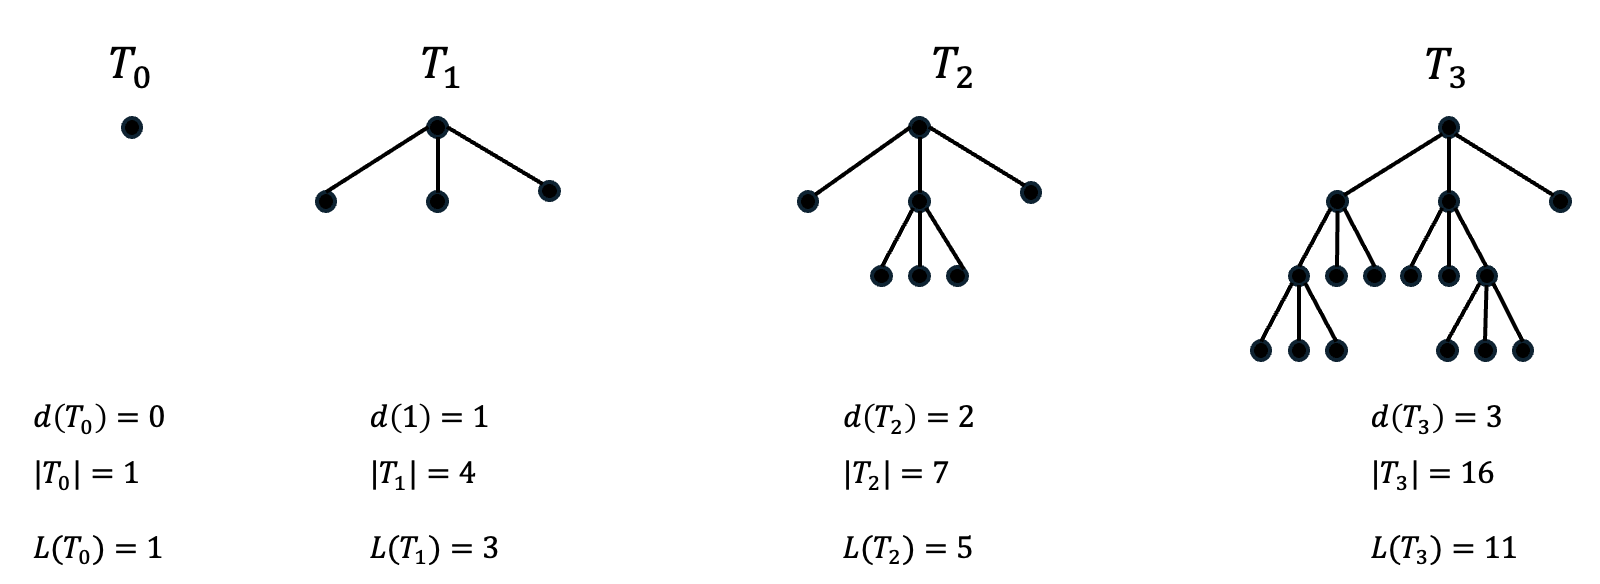
\includegraphics[width=0.8\linewidth]{3_Regular.png}

	\medskip
	\hrule

	\begin{enumerate}[(a)]
		\item State and prove a theorem giving the maximum possible number of leaves
			in a rooted tree of depth $d$ and degree $k$.

		\item State and prove a theorem giving the minimum possible number of leaves
			in a rooted tree of depth $d$ and degree $k$.

		\item State and prove a theorem giving the maximum possible number of nodes in
			a rooted tree of depth $d$ and degree $k$.

		\item State and prove a theorem giving the minimum possible number of nodes in
			a rooted tree of depth $d$ and degree $k$.
	\end{enumerate}

	Note: each of these proofs should be done in two parts. In the first part, a
	bound should be proven by induction. In the second, the bound should be proven
	tight.

	\medskip

	For example, in (a) you should find a function $f(d,k)$ and prove by induction
	that the number of leaves in a rooted tree of depth $d$ and degree $k$ is at
	most $f(d,k).$ An induction proof is necessary here since the trees are
	defined recursively. You should then, for each $d,k$, describe a tree that meets
	those bounds.

	\subsection*{\textbf{Solution:}}
	\begin{enumerate}[(a)]
		\item The max leaves in a rooted tree of depth $d$ and degree $k$ is $L(T)=k^{d}$

		\item The min leaves in a rooted tree of depth $d$ and degree $k$ is $L(T)=(k
			-1)d+1$

		\item $1+k+k^{2}+\cdots+k^{d}$

		\item $kd+1$
	\end{enumerate}

	\newpage
\end{document}